\documentclass[12pt]{article}
\usepackage[margin=1in]{geometry}
\usepackage{mathrsfs}
\usepackage{amsmath}
%\usepackage{mathptmx}    % times with math
%\usepackage{pxfonts}
%\usepackage[sc]{mathpazo}
\usepackage[T1]{fontenc}
\usepackage{subcaption}
\usepackage[font={footnotesize,it}]{caption}
\usepackage{authblk}
\usepackage{lineno}
\usepackage{graphicx}
\linespread{1.15}
\usepackage{fancyhdr}
\pagestyle{fancy}
\lhead{DRAFT}

\newcommand{\nf}[1]{\text{#1}}

\usepackage[
  backend=biber,
  citestyle = authoryear,
  bibstyle = authoryear,
  firstinits=true,
  uniquename=false
  ]{biblatex}
\addbibresource{cfs-model-refs.bib}


\graphicspath{{/home/conor/Dropbox/Leeds_postdoc/Papers/cfs-model/paper/figures/}}

\usepackage{hyperref}
\hypersetup{
  colorlinks=false,
  citecolor=blue
}

% redefine abstract environment
\renewenvironment{abstract}
{\begin{quote}
\small
\noindent \rule{\linewidth}{.5pt}\par{\bfseries \abstractname.}}
{\medskip\noindent \rule{\linewidth}{.5pt}
\end{quote}
}

\usepackage[textfont=it, labelfont=bf]{caption}

\title{A mathematical model of food system security}
\author[1]{Conor Goold}
\affil[1]{Faculty of Biological Sciences, University of Leeds, LS2 9JT, UK}
\author{et al.}
\date{}

\begin{document}
\linenumbers
\modulolinenumbers[5]

\maketitle
\begin{abstract}
  Global food security is threatened by various endogeneous and exogeneous, biotic and abiotic factors, including a rising human population, higher population densities, price volatility and climate change. Perturbations to the global food system have a direct effect on the security and resilience national-level food systems. These effects are felt, in different ways, by both producers, processors and consumers. Various mathematical and computational models exist to understand food systems' responses to shocks and stresses, but most models are tailored to making predictions of specific food systems and are large, high-dimensional models that make uncovering general theoretical food system insights problematic. Here, we present a stylised mathematical model of a national-level food system that incorporates dynamic interactions between domestic production of a food commodity, international trade, domestic demand and consumption, and food commodity price. The model's simplicity allows predicting when domestic production is sustainable when international trade flows are present. Sustainability of domestic production depends on a critical ratio of $i)$ profitability of domestic production to $ii)$ the strength of international trade weighted by the production capacity of domestic production (e.g. capital growth rate and depreciation rates). When the critical ratio exceeds 1, meaning domestic production is sustainable, international imports will either be required to supplement domestic production to meet demand, or domestic production will be profitable enough to produce a surplus of inventory that can be exported. We use the dynamic food systems model to infer the critical parameter values from data from the UK pig industry [...maybe other examples...].\\
\end{abstract}

\newpage
\tableofcontents

\section{Introduction}
Food security is defined as ``when all people at all times have physical and economic access to sufficient, safe and nutritous food to meet their dietary needs and preferences for an active and healthy life'' (\cite{FAO1996}). The realisation of food security depends on the three pillars of access, utilisation and availability (\cite{maxwell1996}; \cite{barrett2010}), and therefore is an outcome of coupled agricultural, ecological and sociological systems (\cite{hammond2012}; \cite{ericksen2008}; \cite{ingram2011}). In recent years, the resilience of food security has become a priority area of research (e.g. \cite{nystrom2019}; \cite{tendall2015}; \cite{bene2016}; \cite{seekell2017}) as biotic and abiotic, endogeneous and exogeneous demands on food systems grow, including the deleterious effects food systems have on their own environments (\cite{springmann2018}; \cite{strzepek2010}). The challenge of food security is for food systems to expand their production capacities while both remaining resilient to unpredictable perturbations and limiting their effects on the environment (\cite{ericksen2010}).

Food system research is inherently transdisciplinary (\cite{drimie2013}; \cite{hammond2012}), of which one strand is computational and mathematical modelling. The utility of quantitative modelling is the ability to build and perturb realistic `systems models' of food systems to project important outcomes, such as food production levels, farmer profitability, envirnomental degradation, food waste, and consumer behaviour (e.g. \cite{springmann2018}; \cite{marchand2016}; \cite{sampedro2020}; \cite{suweis2015}; \cite{scalco2019}; \cite{allen2016}). The difficulty in modelling food systems is their complexity, frequently resulting in large models with tens to hundreds of parameters and variables, which are challenging to analyse and even more challenging to statistically estimate from noisy real-world data. In contrast, a handful of authors have used relatively simple, theoretical models that are more amenable to formal analysis, and have fewer parameters to estimate from data sources, to understand the activities of food systems. For example, \textcite{suweis2015} link population dynamics to food availability and international trade using a generalised logistic model. \textcite{tu2019} recently reported that the global food system is approaching a critical point deliminating collapse into an unsustainable regime by condensing the multi-dimensional global food trade network into a bistable one-dimensional system (using the framework of \cite{gao2016}). Simple models of coupled ecological, economic and agricultural processes have also been investigated. For instance, \textcite{ngonghala2017} explain the emergence of poverty traps, which have direct effects on individual's access to food, by coupling differential equations of human poverty, human disease, and economic growth.

Simplified models of complex systems elicit causal explanations and generate hypotheses of how systems work (\cite{smaldino2017}; \cite{smaldino2019}; \cite{otto2020}). Such \textit{stylised} models are staples of scientific disciplines such as ecology (\cite{may1973}), evolutionary biology (\cite{boyd2003}), epidemiology (\cite{kermack1927}), economics (\cite{nerlove1958}), and physics (\cite{strogatz1994}). Food systems research, however, lacks such foundational models. A potential candidate is research on commodity production cycles that has developed models to couple agricultural production, supply chains, consumer demand, price and human decision-making, such as \textcite{meadows1971}. These approaches have inspired systems dynamics modelling of general commodity and business cycles (\cite{sterman2000}). However, applications of systems dynamics models of commodity cycles are frequently high dimensional, encoding multiple modes of behaviour that are not easily amenable to standard mathematical analysis. Gaining greater theoretical insight into the dynamics of food systems and food security would be aided by simpler models of coupled agri-food systems.

In this paper, we develop and analyse a stylised model of a food system inspired by the systems dynamics modelling of \textcite{meadows1971} and \cite{sterman2000}, but simple enough to offer general theoretical results. To limit our scope, we focus on modelling a national-level food system, where the effects of international trade on domestic production is examined. Like the stylised models used to understand the causal processes in evolution, epidemics, and ecological interactions, our approach necessarily ignores many important features of real food systems. Nonetheless, the simplicity of our model allows us to elucidate the precise conditions under which different stable modes of behaviour important to food security emerge in our system.

We apply our theoretical model to the case of the UK pig industry. Historically, pig industries have been of much interest to economists and agronomists as one of the first investigations into business or `pork' cycles (\cite{haldane1934}; \cite{coase1935}; \cite{ezekiel1938}; \cite{harlow1960}; \cite{meadows1971}; \cite{zawadzka2010}; \cite{parker2014}; \cite{sterman2000}). Business cycles reflect the oscillations between commodity prices and supply, which have been posited to be the result of both endogeneous (e.g. \cite{nerlove1958}) and exogeneous mechanisms (e.g. see \cite{gouel2012}). In the last 20 years, the size of the UK pig industry has decreased markedly due to a combination of legislative, epidemiological, and trade-related issues (\cite{taylor2006}; \cite{dawson2009}). For example, in 1997, the UK breeding herd comprised around 800,000 sows, and domestic production exceeded imports. Following the ban on sow gestation crates in 1999, as well as disease outbreaks in the early 2000s, imports of pig meat increased by 50\% (\cite{DEFRApigcattlestats2020}), exceeding domestic production. While domestic production currently accounts for around 60-65\% of total supply (\cite{DEFRApigcattlestats2020}), the UK pig industry is still at risk from high costs of production (\cite{BPEXprofitability2011}) and `opportunistic dealing' within the pork supply chain favouring cheaper imports (\cite{bowman2013}). The sustainability of the UK pig industry is, thus, a prime concern for UK food security. As well as insights into the sustainability of the UK pig industry, we illustrate limitations of our stylised model for modelling real-world data sources.

\section{Materials and methods}

\subsection{Theoretical model}
Our food system model is composed as a system of coupled ordinary differential equations, with the state variables of capital, inventory, consumer demand, and price. The general structure of our model is presented in Figure \ref{fig_cfs}, and Table \ref{t_symbols} provides the exact variable parameter definitions. Capital represents a raw component used to gauge the viability of the domestic industry, which could represent, for instance, the number of animals in the breeding herd for meat industries (e.g. \cite{meadows1971}), the number of paddy fields in rice supply chains (e.g. \cite{chung2018}), or infrastructure or equipment in neoclassical economic growth models (\cite{ngonghala2017}). Inventory is the stock of processed food commodity being investigated. Customer demand represents the amount of inventory demanded per time unit by the population of consumers. The commodity price represents the price received by producers per unit of commodity produced, and is taken to be directly proportional to the price presented to consumers (i.e. we do not account for retail mark-ups on price). While many of the mechanisms in supply chain functioning may be represented as a disrecte-time system, we assume the aggregate behaviour of the national-level food system is adequately approximated in continuous time by a system of differential equations.

\begin{figure}[t!]
  \centering
  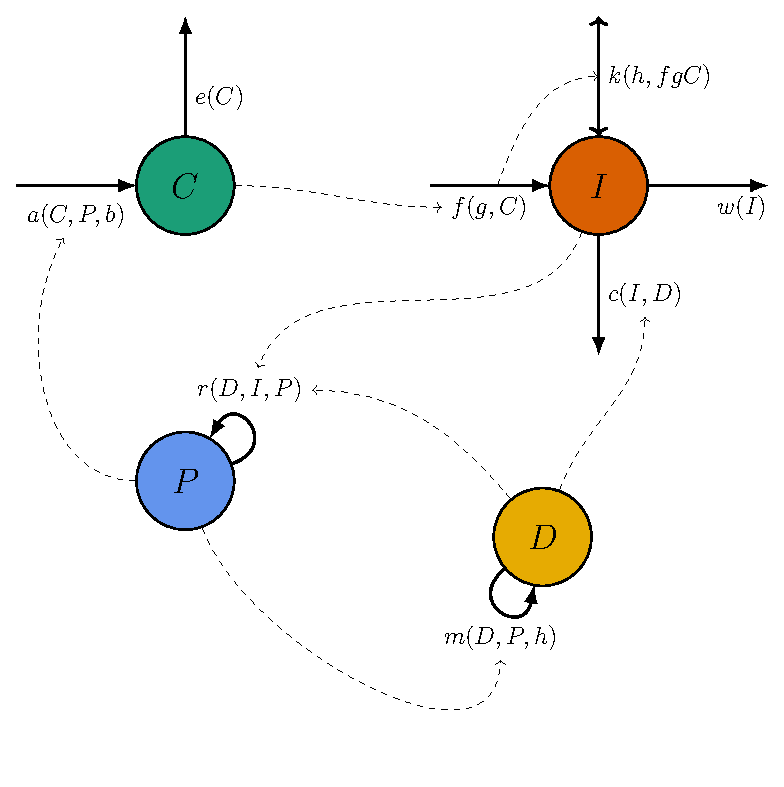
\includegraphics[scale=0.8]{figure_1.pdf}
  \caption{The general structure of the theoretical complex food system model. Blue circles denote the rates of change of the four state variables (capital, inventory, demand and price). Solid arrows indicate the different flows into and out of each state variable as generic functions of the model state variables and parameters. Dashed arrows show dependencies between different state variables and flows.}
  \label{fig_cfs}
\end{figure}

Capital changes according to the equation:
%
\begin{equation}
  \frac{dC}{dt} = a C \Big(\frac{P}{b} - 1\Big) - e C \quad, \quad C(0) = C_0
  \label{eq_capital}
\end{equation}
%
with initial condition at $t = 0$, $C_0$. The parameter $a$ is the rate of capital change (increase or decrease) depending on the price to production cost ($b$) ratio. Captial depreciates at a per-capital rate $e$, which can be interpreted as the inverse of the average life-time of capital (see supplementary materials for derivation).

Inventory changes according to:
%
\begin{equation}
  \frac{dI}{dt} = f g C - w I - \frac{I}{sD + I} D + k (h - f g C) \quad, \quad I(0) = I_0
  \label{eq_inventory}
\end{equation}
%
The first term represents the amount of inventory generated by domestic capital per time unit (i.e. domestic production), where $f$ is a production rate, and $g$ is a conversion factor representing the amount of inventory units produced per unit of capital. Inventory is wasted at rate $w$. The third term denotes the rate of inventory consumption by consumers, which is a non-linear Holling type-II/Michaelis-Menten function asymptoting at $I$ for $D >> I$. The function $I/(sD + I)$ can be interpreted as the proportion of the demand that can be satisfied with the current inventory level. The parameter $s$ is the `reference coverage': the number of time units-worth of inventory processors desire to have in-stock. Perishable food commodities (e.g. meat) will have a lower reference coverage, whereas less perishable items (e.g. rice, flour) can be stored for longer periods and, therefore, processors can control stock levels by increasing $s$, lowering the proportion of demanded units satisfied.

The final term in equation \ref{eq_inventory} represents international trade, and its formulation can communicate different dynamics between domestic producers, processors and retailers. We retain simplicity by assuming that trade is proportional to the difference between reference demand ($h$) and current domestic production ($f g C$). When $h > f g C$, inventory is imported, and when $h < f g C$, inventory is exported. Because actual demand is a function of both $h$ and price, processors adapt their trade levels to the demand expected if all else were equal (e.g. the current commodity is just as attractive as competing substitute items). In some industries, such as the UK pig industry, cheaper international imports lower the domestic commodity price (\cite{AHDBeuroexhange2015}), and thus processors can import more items when demand drops below the reference demand level and domestic production is insufficient. The parameter $k$ controls the proportion of the difference between the reference demand and current domestic production that can be imported/exported. This is a placeholder for more complex mechanisms that could influence the volumes of trade (e.g. see \cite{tu2019}), such as the effects of trade tariffs, or the costs of production of commodities in trade partner countries.

The instantaneous rate of change in demand is modelled as a simple function of reference demand and the commodity price to reference price ratio:
%
\begin{equation}
  \frac{dD}{dt} = m \Big( h \frac{q}{p} - D\Big) \quad, \quad D(0) = D_0
  \label{eq_demand}
\end{equation}
%
The parameter $m$ controls the time-responsiveness of demand. The reference price $q$ is typically interpreted as the price of substitute items (\cite{sterman2000}) or could represent customer's willingness to pay. In any case, when the current price exceeds the reference price, demand falls, and vice versa.

Many models exist for describing the price of commodities (e.g. see \cite{legrand2019} or \cite{deGoede2013} for some examples), and we adopt a relatively simple formulation here that has the rate of change of price depend only on the coverage:
%
\begin{equation}
  \frac{dP}{dt} = r P \Big(\frac{sD}{I} - 1\Big) \quad, \quad P(0) = P_0
  \label{eq_price}
\end{equation}
%
The coverage is a dimensionless quantity representing the amount of inventory needed to sustain current demand for $s$ time periods divided by the current inventory level. At rate given by $r$, the price increases when the coverage exceeds one, $sD/I > 1$, and decreases when coverage falls below $1$.

\begin{table}[t!]
  \centering
  \footnotesize
  \begin{tabular}{p{2cm}p{5cm}p{2cm}}
    \textbf{Symbol} & \textbf{Definition} & \textbf{Units} \\ \hline
    \textit{Variables} &&\\
    $C$    & Capital             & [$C$]\\
    $I$    & Inventory           & [$I$]\\
    $D$    & Demand              & [$It^{-1}$]\\
    $P$    & Price               & [$PI^{-1}$]\\
    $t$    & Time                & [$t$]\\
    \textit{Parameters} &&\\
    $a$    & Capital growth rate & [$t^{-1}$]\\
    $b$    & Cost of capital production & [$PI{-1}$]\\
    $e$    & Capital depreciation rate & [$t^{-1}$]\\
    $f$    & Capital production rate & [$t^{-1}$]\\
    $g$    & Capital conversion factor & [$IC^{-1}$]\\
    $w$    & Inventory waste rate     & [$t^{-1}$]\\
    $s$    & Reference coverage       & [$t$]\\
    $k$    & Maximum trade proportion        & [$-$]\\
    $h$    & Reference demand         & [$It^{-1}$]\\
    $m$    & Demand response rate     & [$t^{-1}$]\\
    $q$    & Reference price          & [$PI^{-1}$]\\
    $r$    & Price growth rate        & [$t^{-1}$]\\\hline
  \end{tabular}
  \caption{Symbols, definitions and their units for the complex food system model.}
  \label{t_symbols}
\end{table}

To make our model more generalisable, we non-dimensionalise the system of equations above (see supplmentary materials for non-dimensionalisation) using the dimensionless quantities in Table \ref{t_nd_symbols}, which reduces the number of parameters from 12 to 8. The non-dimensionalised system of equations is:

\begin{equation}
  \frac{dv}{d\tau} = v \Big(\alpha z - 1\Big) - \beta v
\end{equation}

\begin{equation}
  \frac{dx}{d\tau} = \delta v - \omega x - \gamma \frac{xy}{y + x} + \kappa ( \gamma - \delta v)
\end{equation}

\begin{equation}
  \frac{dy}{d\tau} = \mu \Big( z^{-1} - y\Big)
\end{equation}

\begin{equation}
  \frac{dz}{d\tau} = \rho z\Big(\frac{y}{x} - 1\Big)
\end{equation}
%
where $\{v, x, y, z\}$ now represent the dimensionless state variables, $\tau$ is rescaled time, and the dimensionless parameter groups are denoted by Greek letters.

\begin{table}[t!]
  \centering
  \footnotesize
  \begin{tabular}{p{2cm}p{2cm}p{7cm}}
    \textbf{Symbol} & \textbf{Definition} & \textbf{Description} \\ \hline
    \textit{Variables} &\\
    $v$  & $\frac{C}{C_0}$    & Rescaled capital        \\
    $x$  & $\frac{I}{hs}$  & Rescaled inventory      \\
    $y$  & $\frac{D}{h}$  & Rescaled demand             \\
    $z$  & $\frac{P}{q}$  & Rescaled price               \\
    $\tau$  & $\frac{t}{1/a}$  & Rescaled time\\
    \textit{Parameters} &\\
    $\alpha$   & $q/b$  & Reference price compared to cost of production\\
    $\beta$    & $e/a$  & Capital depreciation rate compared to its growth rate\\
    $\delta$    & $f g C_{0}/(ahs)$ & Initial capital production compared to expected demand per capital growth rate\\
    $\omega$    & $w/a$ & Inventory waste rate compared to capital growth rate\\
    $\gamma$    & $1/(as)$ & Inverse of captial growth rate over reference coverage\\
    $\kappa$    & $k$    & Maximum import proportion of reference demand\\
    $\mu$       & $m/a$  & Demand change rate compared to capital growth rate\\
    $\rho$      & $r/a$  & Price change rate compared to capital growth rate\\
    \hline
  \end{tabular}
  \caption{Symbols and definitions for the dimensionless complex food system model.}
  \label{t_nd_symbols}
\end{table}

\subsection{Data sources \& parameter estimation}
A range of data is collected on the UK pig industry, but raw time series data is only available for certain variables and time frames. To fit our theoretical model, we focused on monthly data over a period of 5 years from 2015 to 2020, which covers the available data for prices per kilogram of deadweight (the `pig price'). Monthly pig prices were accessed through the Deparment for Environment, Food and Rural Affairs (DEFRA) webpage (\cite{DEFRAlivestockprices}), along with the June and December surveys of the size of breeding herd (\cite{DEFRAlivestocknumbers}). Monthly data for the inventory of pork, taking into account consumption and waste, is not reported in the UK. While customer demand is a theoretical quantity, we used the total monthly supplies of pig meat, calculated as domestic production of pig meat plus imported pig meat minus exported pig meat, as an indication of customer demand levels per month. Monthly data for UK production of pig meat was accessed from DEFRA (\cite{DEFRApigcattlestats2020}), while monthly imports and exports of pig meat was accessed from the Agricultural and Horticultural Development Board (\cite{AHDBpigmeatrade}). Missing data was considered missing completely at random (i.e. ignorable) because the missing data was not assumed to impact the accuracy of the available data.

The parameters and initial conditions of the non-dimensionalised model were estimated using Bayesian estimation in the probabilistic programming language Stan (\cite{carpenter2017}) using the RStan interface in R (\cite{stan2019}; \cite{rcoreteam2020}) using Stan's Runge-Kutta 4th and 5th order integration scheme (see Stan code in the supplementary materials). The available monthly time series data, $Y$, for month $i$ state variable $j$ was assumed log normal distributed:

\begin{equation}
  Y_{i}^{j} \sim \text{Lognormal}( ln( Z^{j} ), \sigma^{j})
\end{equation}
%
where $Z^{j}$ is the state variable computed from the food systems model. In addition to fitting the state variables of the model to the time series data, we fit the UK monthly production figures, and the monthly imports and exports, to the respective flows from the model:

\begin{equation}
  \text{Production} \sim \text{Lognormal}( ln( f g Z^{1} ), \epsilon_{1})
\end{equation}

\begin{equation}
  \text{Imports} \sim \text{Lognormal}( ln( k h ), \epsilon_{2})
\end{equation}

\begin{equation}
  \text{Exports} \sim \text{Lognormal}( ln( k f g Z^{1} ), \epsilon_{3})
\end{equation}


To aid computation, all parameters were transformed to a similar scale and given $\text{Normal}(0, 1)$ prior distributions, and were back-transformed to the appropropriate scale when integrating the model. We ran 4 Markov chain Monte Carlo (MCMC) chains consisting of 2,500 iterations of warmup and 2,500 iterations of sampling, providing 10,000 samples from the posterior distribution for inference. All chains ran without any divergent transitions, and all parameters had effective sample sizes $>> 1000$ and $\hat{R}$ statistics (i.e. the Gelman-Rubin diagnositc) $0.99 < \hat{R} < 1.002$ indicating convergence.


\section{Results}

\subsection{Model analysis}
While the mechanisms represented by the model are simple, it still comprises a four dimensional system of non-linear equations, of which there are no explict solutions. Nontheless, its dynamics can be summarised by investigating its stable modes of behaviour. To investigate stability, we conduct linear stability analyses (\cite{strogatz1994}). Linear stability analysis is based on a Taylor series expansion in multiple variables around the fixed points ($\{\hat{v}, \hat{x}, \hat{y}, \hat{z}\}$), where asymptotic (i.e. $t \rightarrow \infty$) stability to small perturbations can be inferred when the real part of the eigenvalues of the system's matrix of partial derivatives (the Jacobian matrix representing the linearisation around the fixed points) evaluated at each equilibrium are negative. Notably, the inverse of the leading eigenvalue of the Jacobian matrix determines the `characteristic return time' of the system, with more resilient systems returning more quickly to their equilibria following a disturbance (\cite{pimm1984}).

\subsubsection{Without international trade}
When international trade is not present (i.e. $\kappa = 0$), there is one stable fixed point of the system given by the state variable values $\big \{\frac{\alpha(2\omega + \gamma)}{2 \delta (1 + \beta)}, \frac{\alpha}{1 + \beta}, \frac{\alpha}{1 + \beta}, \frac{1 + \beta}{\alpha}\big\}$. Another fixed point is where all state values are 0 (i.e. no industry). Conducting a linear stability analysis around the the latter fixed point, the eigenvalues of the Jacobian matrix at this equilibria are $\{(-1 - \beta), - \omega, - \mu, - \rho)\}$.
Because all parameters are defined to be positive (except $\kappa$, which is $0$ here), there are no conditions where the `no industry' equilibria will be stable when international trade is absent. In other words, the domestic industry is always viable.

\iffalse
The Jacbobian matrix ($\boldsymbol{J}$) at this equilibria evalutes to:

\begin{equation}
  \boldsymbol{J} \Big |_{\{\frac{\alpha(2\omega + \gamma)}{2 \delta (1 + \beta)}, \frac{\alpha}{1 + \beta}, \frac{\alpha}{1 + \beta}, \frac{1 + \beta}{\alpha}\}} =
  \begin{pmatrix}
    0   &    0     &  0 &  \frac{\alpha^2(2 \omega + \gamma)}{2 \delta (1 + \beta)} \\
    \delta & - \omega - \frac{\gamma}{4}  &  - \frac{\gamma}{4} & 0 \\
    0      &           0            & -\mu     & - \mu (\frac{\alpha}{1+\beta})^2\\
    0      &   - \rho (\frac{1 + \beta}{\alpha})^2    & \rho (\frac{1+\beta}{\alpha})^2 & 0 \\
  \end{pmatrix}
\end{equation}
\fi

\subsubsection{With international trade}
When $0 < \kappa < 1$, international trade is possible, opening the possibility of competition between domestic and international products, or of an export market for domestic production. An unstable equilibria still exists where all state variables are 0. However, in addition, there is 1) an unsustainable domestic production equilibrium, where the food system is viable overall through complete reliance on international imports, and 2) a sustainable domestic production equilibrium, where the profitability of the domestic industry is high enough to compete with international trade.

The unsustainable domestic production equilibria is given by the set of fixed points $\{0, \frac{\kappa \gamma}{\omega + \frac{\gamma}{2}}, \frac{\kappa \gamma}{\omega + \frac{\gamma}{2}}, \frac{\omega + \frac{\gamma}{2}}{\kappa \gamma}\}$. The Jacbobian matrix ($\boldsymbol{J}$) at this equilibria evalutes to:

\begin{equation}
  \boldsymbol{J} \Big |_{\big \{0, \frac{\kappa \gamma}{\omega + \frac{\gamma}{2}}, \frac{\kappa \gamma}{\omega + \frac{\gamma}{2}}, \frac{\omega + \frac{\gamma}{2}}{\kappa \gamma}\big \}} =
  \begin{pmatrix}
    \frac{\alpha(\omega + \frac{\gamma}{2})}{\kappa \gamma} - 1 - \beta   &    0     &     0    &  0 \\
    \delta (1 - \kappa) & - \omega - \frac{\gamma}{4}  &  - \frac{\gamma}{4} & 0 \\
    0      &           0            & -\mu     & - \mu (\frac{\kappa \gamma}{\omega + \frac{\gamma}{2}})^2\\
    0      &   - \rho (\frac{\omega + \frac{\gamma}{2}}{\kappa \gamma})^2    & \rho (\frac{\omega + \frac{\gamma}{2}}{\kappa \gamma})^2 & 0 \\
  \end{pmatrix}
\end{equation}
%
and its eigenvalues ($\boldsymbol{\lambda}$) are the roots of the fourth-degree characteristic polynomial:

\begin{equation}
  \Big(\frac{\alpha(\omega + \frac{\gamma}{2})}{\kappa \gamma} - 1 - \beta - \lambda\Big) \Big[ - \lambda^3 + \big(-\omega - \frac{\gamma}{4} - \mu\big) \lambda^2 + \big(- \mu(\omega + \rho) - \frac{\gamma}{4}\big) \lambda - \frac{\gamma}{2} \mu \rho\Big] = 0
\end{equation}
%
The first eigenvalue can be determined directly as:

\begin{equation}
  \lambda_{1} = \frac{\alpha(\omega + \frac{\gamma}{2})}{\kappa \gamma} - 1 - \beta
\end{equation}
%
By using the Routh-Hurwitz conditions, the sign of the remaning eigenvalues' real parts (\cite{ottoday2011}) will always be negative (see the supplementary materials). Ultimately, the unsustainable domestic production mode will be stable if:

\begin{equation}
  \frac{ \alpha (\omega + \frac{\gamma}{2})}{\kappa \gamma(1+\beta)} < 1
\end{equation}
%
The previous `critical ratio' can be loosely interpreted as a balance between $i$) the profitability of domestic production, weighted by both the wastage rate and capital growth rate, and $ii$) the strength of international trade, weighted by the domestic capital growth rate and domestic capital depreciation rate. The most influential parameters dictating the critical ratio's value are $\alpha$, $\kappa$ and $\beta$ (see Figure S1), where increases in $\alpha$ (the ratio of reference price to cost of production) increase the critical ratio, but increases in $\kappa$ (strength of trade) and $\beta$ (capital depreciation rate to growth rate ratio) decrease the critical ratio. Figure 1a illustrates the bifurcation diagram of the dimensionless capital state variable as a function of $\alpha$.

\begin{figure}[t!]
  \begin{subfigure}{0.5\textwidth}
      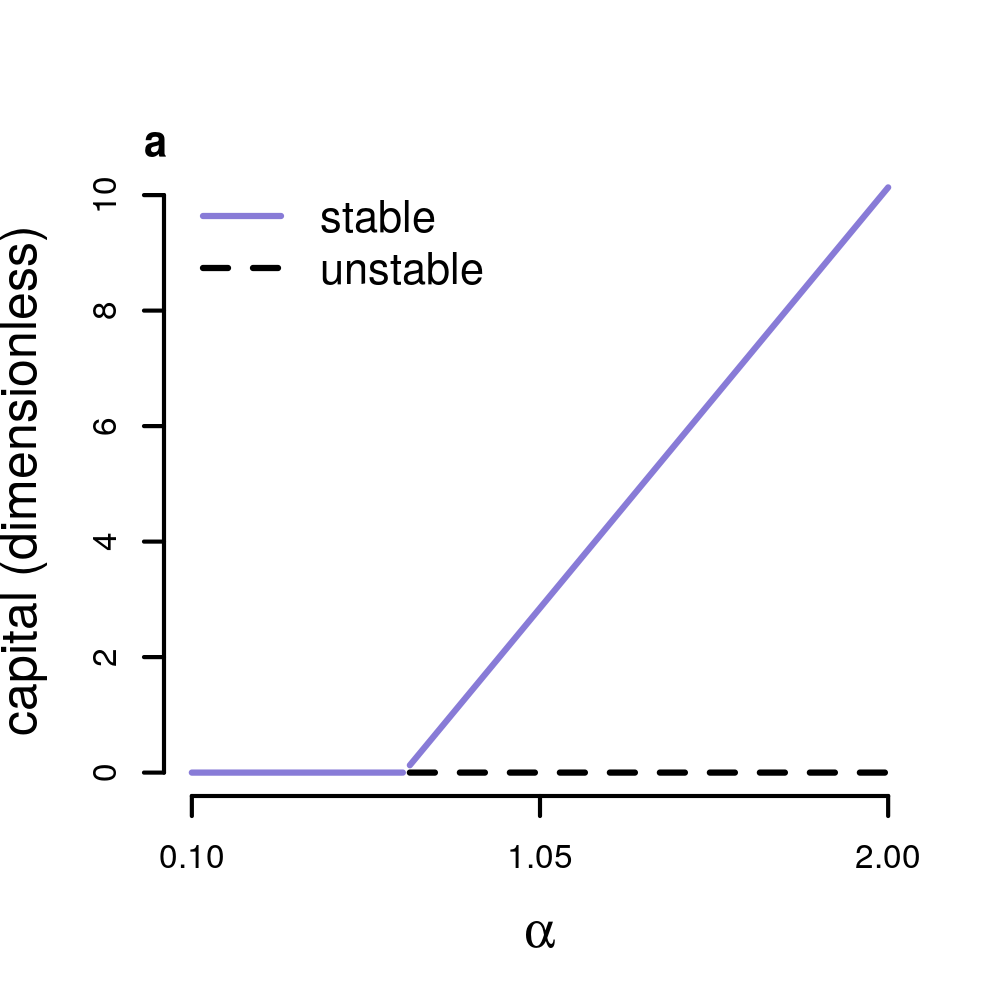
\includegraphics[scale=0.6]{figure_2a.png}
  \end{subfigure}%
  ~%
  \begin{subfigure}{0.5\textwidth}
      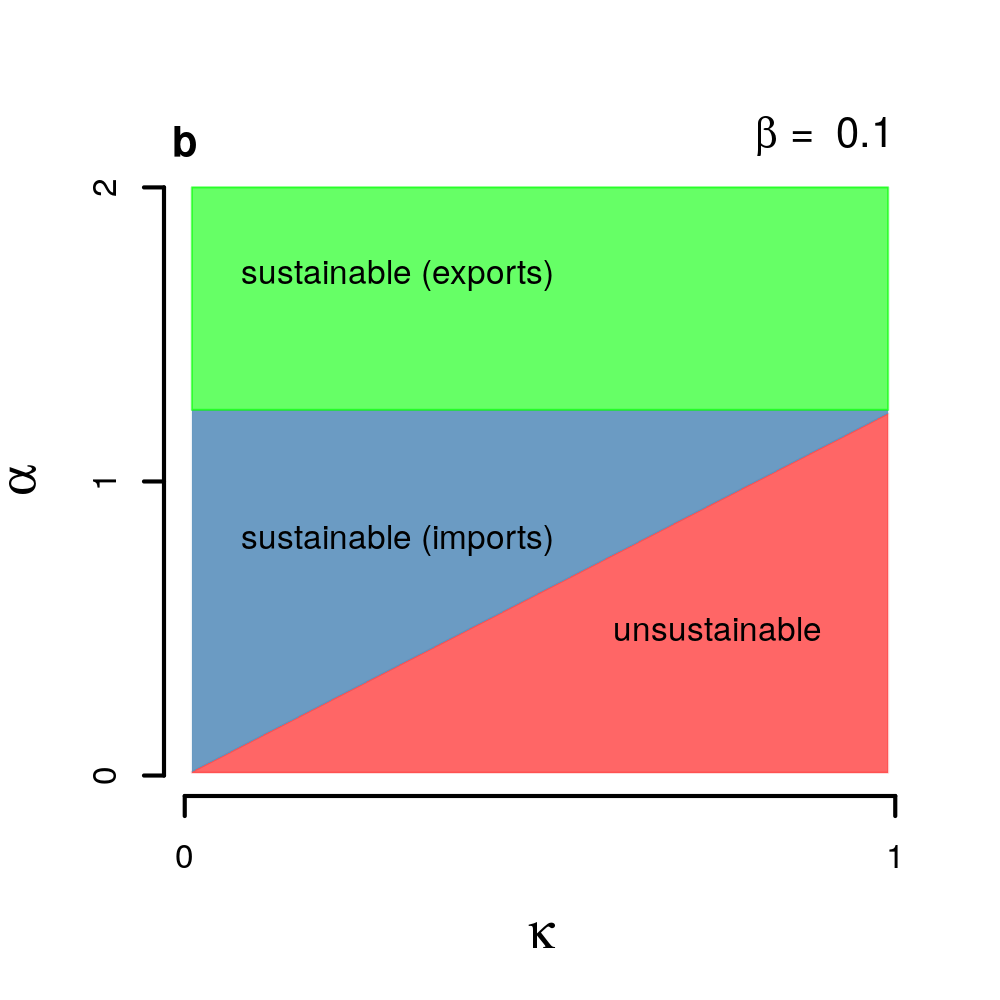
\includegraphics[scale=0.6]{figure_2b.png}
  \end{subfigure}

  \begin{subfigure}{0.5\textwidth}
      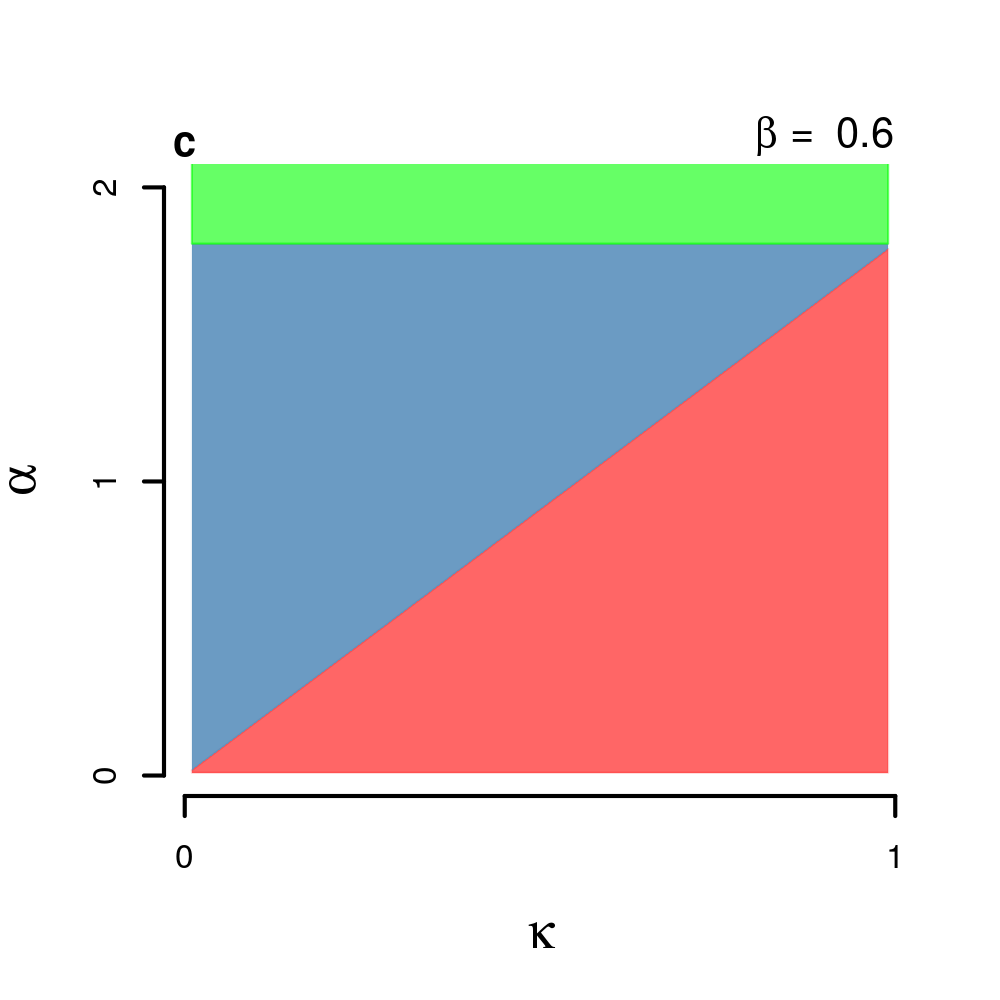
\includegraphics[scale=0.6]{figure_2c.png}
  \end{subfigure}%
  ~%
  \begin{subfigure}{0.5\textwidth}
      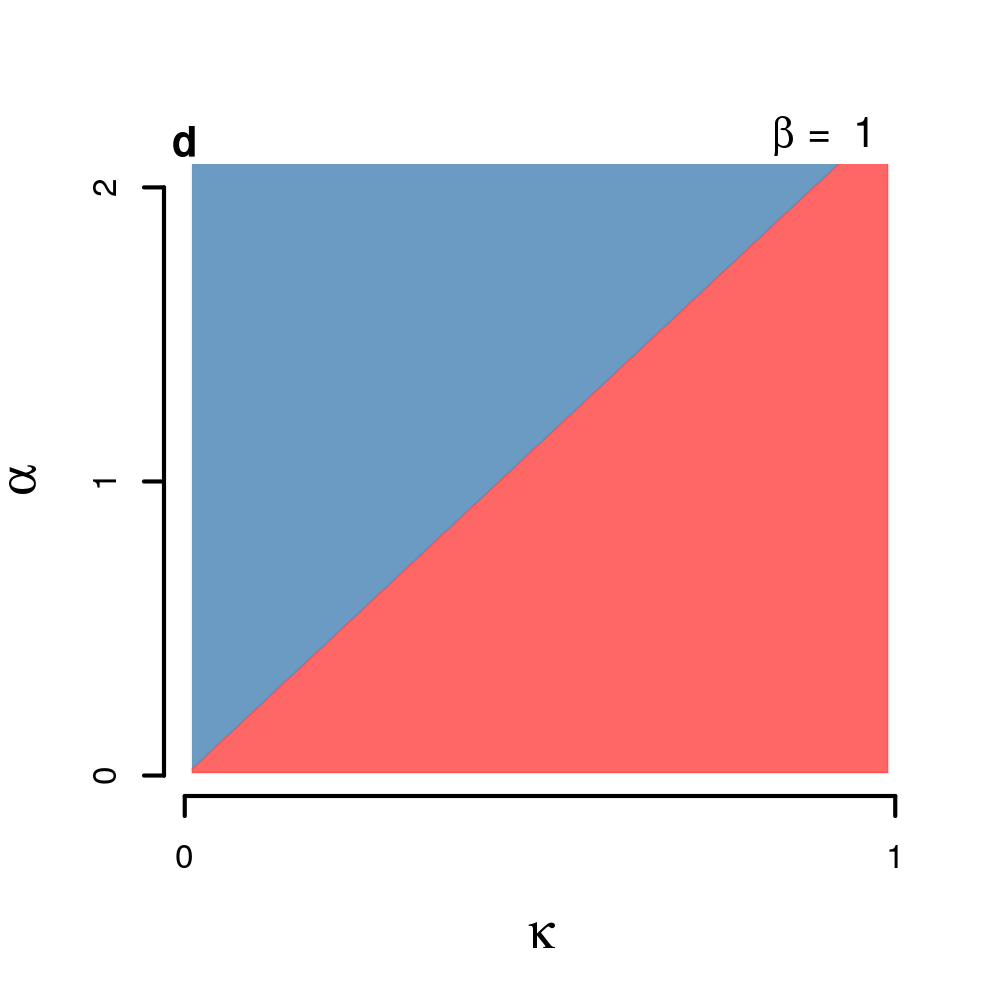
\includegraphics[scale=0.6]{figure_2d.png}
  \end{subfigure}%

  \caption{Stable modes of the model incorporating international trade ($0 < \kappa < 1$). Panel a shows the bifurcation diagram between stable (solid blue) and unstable (dashed black) behaviours (with $\beta$, $\gamma = 26$, $\omega = 10$, $\kappa = 0.5$, $\delta = 5$). Panels b-d show the stable modes of behaviour in ($\kappa, \alpha$) space for differing values of $\beta$ (b = 0.1, c = 0.6, d = 1), distinguishing between unsustianable (red), sustainable with imports (blue), and sustainable with exports (green) behaviours. Panels b-d are produced with the remaining parameters at $\gamma = 26$, $\omega = 10$ and $\delta = 5$.}
  \label{figure2}
\end{figure}

When the critical ratio exceeds 1, the sustainable domestic production equilibrium is given by $\{\frac{2 \gamma \kappa (- 1 - \beta) + \alpha (\gamma + 2 \omega)}{2 \delta (1+\beta)(1 - \kappa) }, \frac{\alpha}{1 + \beta}, \frac{\alpha}{1 + \beta}, \frac{1 + \beta}{\alpha}\}$. In the latter case, the equilibrium values of inventory, demand and price are the same as the equilibrium values of the model without international trade (see above), determined by the profitability of the domestic industry and the ratio of capital depreciation and growth rates. The equilibrium value of capital is similar to the equilibrium value found in the model without international trade, but now increased by both the odds of international trade (i.e. $\frac{\kappa}{1-\kappa}$) but decreased by the term $ - 1 - \beta$, which is always negative for $\beta > 0$.
The two equilibria are equal when $\kappa = 0$. Thus, if the critical ratio $> 1$ and domestic production is sustainable, trade strength alone has a positive effect on domestic capital keeping other parameters constant.

The latter result can also be viewed as a balance between two separate modes of behaviour: either domestic production will produce a surplus of inventory, allowing exports of domestic capital dependent on the value of $\kappa$, or domestic inventory needs to be supplemented by international imports to meet demand. Domestic capital will produce a surplus when $\frac{\gamma}{\delta} - \hat{v} < 0$, or when:

\begin{equation}
  \alpha > \frac{2 \gamma (1 + \beta)}{\gamma + 2 \omega}
\end{equation}
%
Figures 1b-d demonstrate the relationship between the sustainable and unsustainable stable modes of behaviour in $(\kappa, \alpha)$ space for differing values of $\beta$, as well as the distinction between the sustainable state supplemented by imports, and the sustainable state requiring domestic production to be exported.

\subsection{Application to UK pig industry}
The parameter estimates for $a$, $k$ and $q$ are given in Table \ref{table_parameter_estimates}, and how the model results compare to the raw data is shown in Figure X. There is large uncertainty in the estimates, which is induced both by the tolerance thresholds for the ABC-MCMC algorithm, $\epsilon$, and because the amount of data available is relatively small to inform the parameter values. Importantly, the critical ratio is plausibly above 1 (although its 95\% HDI approaches 1) suggesting that the the UK pig industry is currently sustainable.

\begin{table}[t!]
  \centering
  \footnotesize
  \begin{tabular}{p{5cm}p{2cm}p{3cm}p{2cm}p{2cm}}
    \textbf{Parameter} & \textbf{Mean} & \textbf{95\% HDI} & \textbf{ESS} & \textbf{$\hat{R}$} \\ \hline
    $a$ &  & [] &  & \\
    $b$ &  & [] & & \\
    $q$ &  & [] &  & \\
    critical ratio &  & [] & & \\
  \end{tabular}
  \caption{Key parameter estimates (mean and 95\% highest density interval, HDI) and effective sample sizes (ESS) from fitting the model to the UK pig industry data.}
  \label{table_parameter_estimates}
\end{table}

\begin{figure}[t!]
  \begin{subfigure}{0.5\textwidth}
    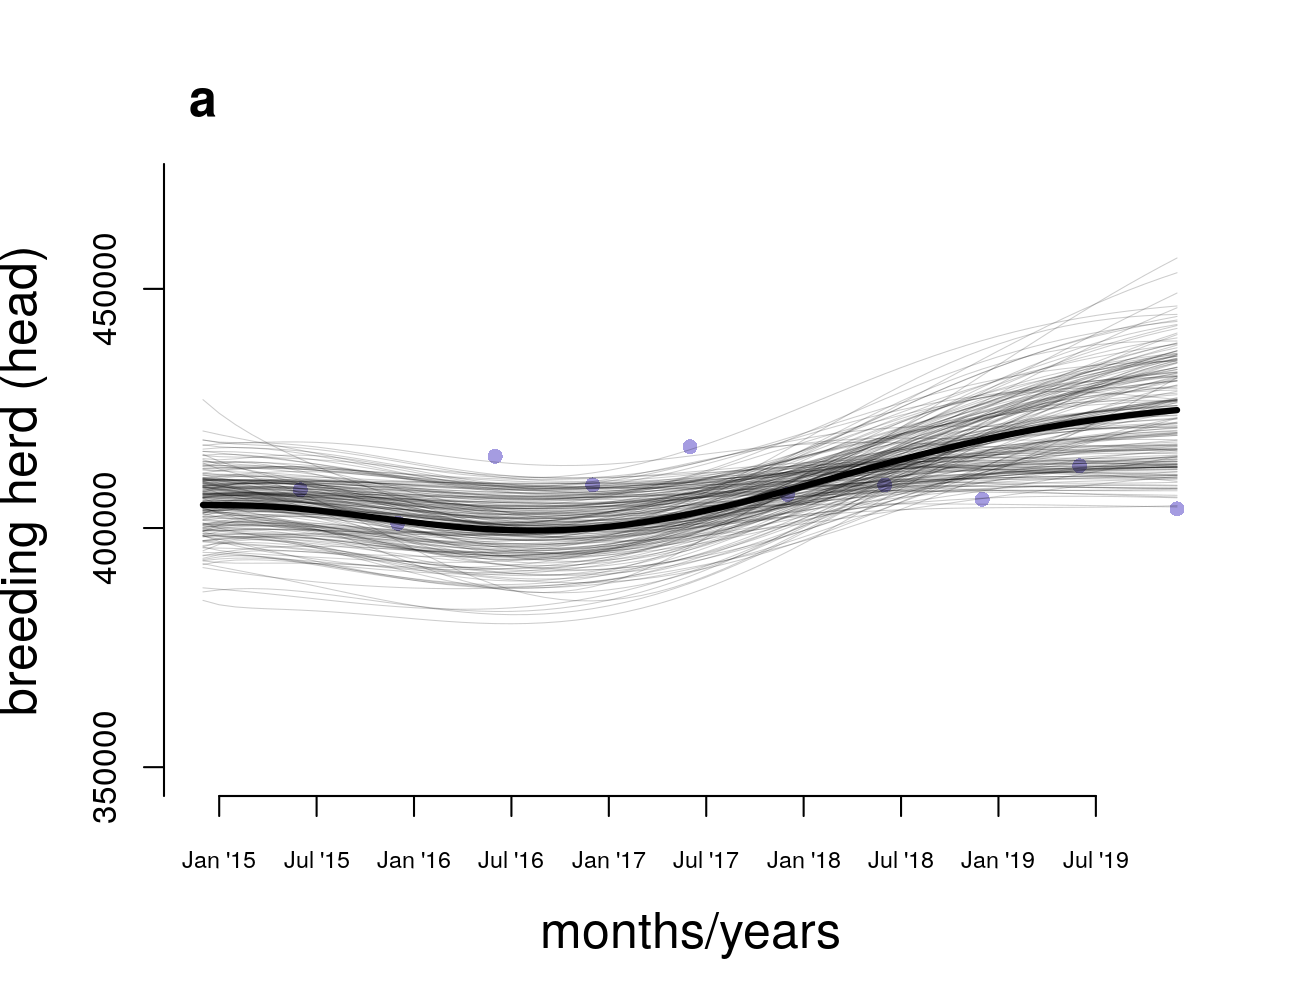
\includegraphics[scale=0.5]{figure_3a.png}
  \end{subfigure}%
  %~
  \begin{subfigure}{0.5\textwidth}
    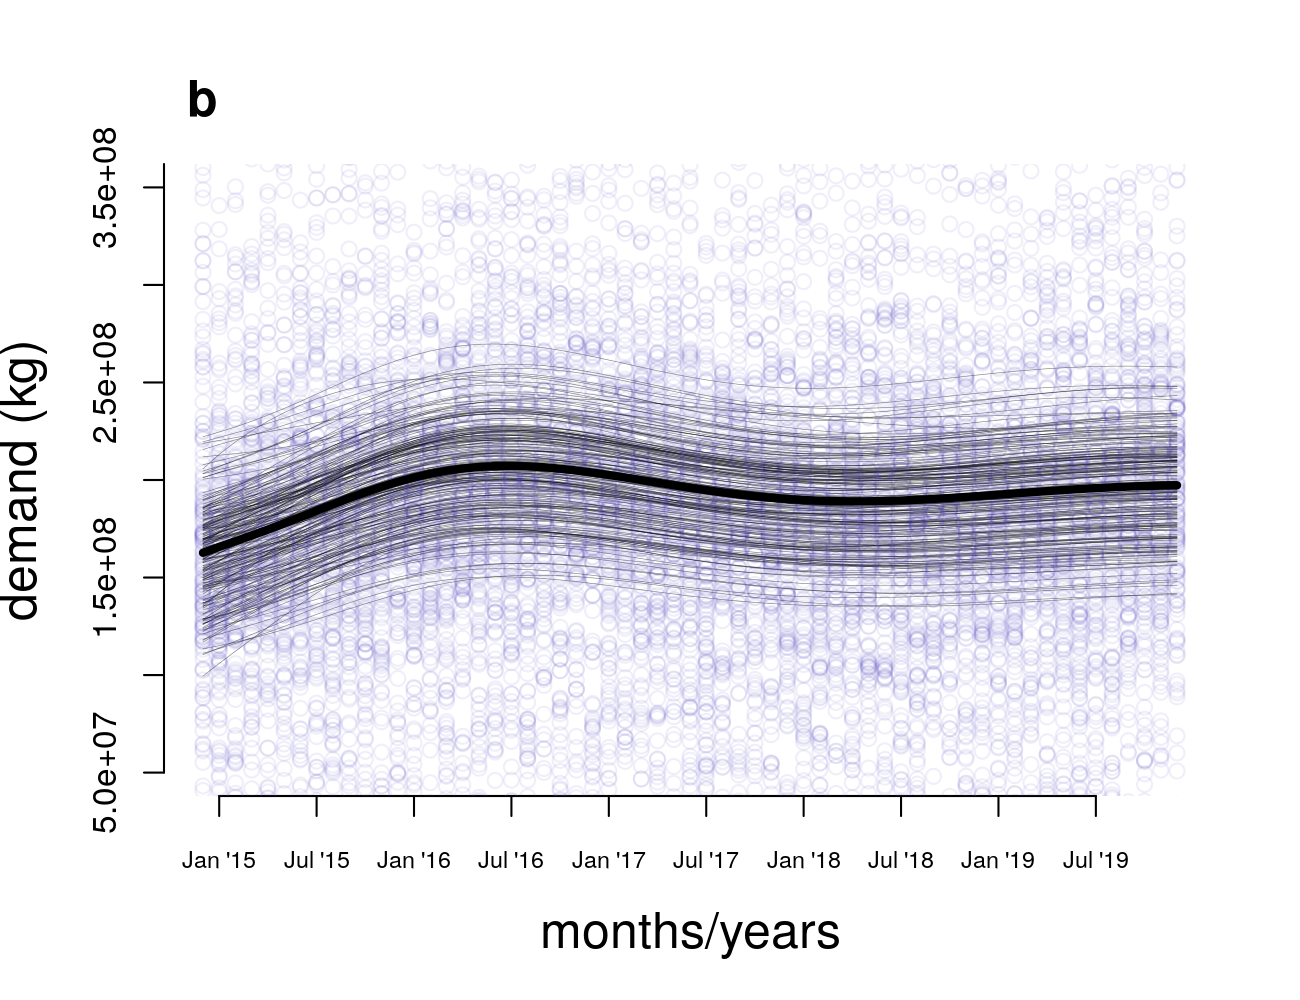
\includegraphics[scale=0.5]{figure_3b.png}
  \end{subfigure}

  \begin{subfigure}{0.5\textwidth}
    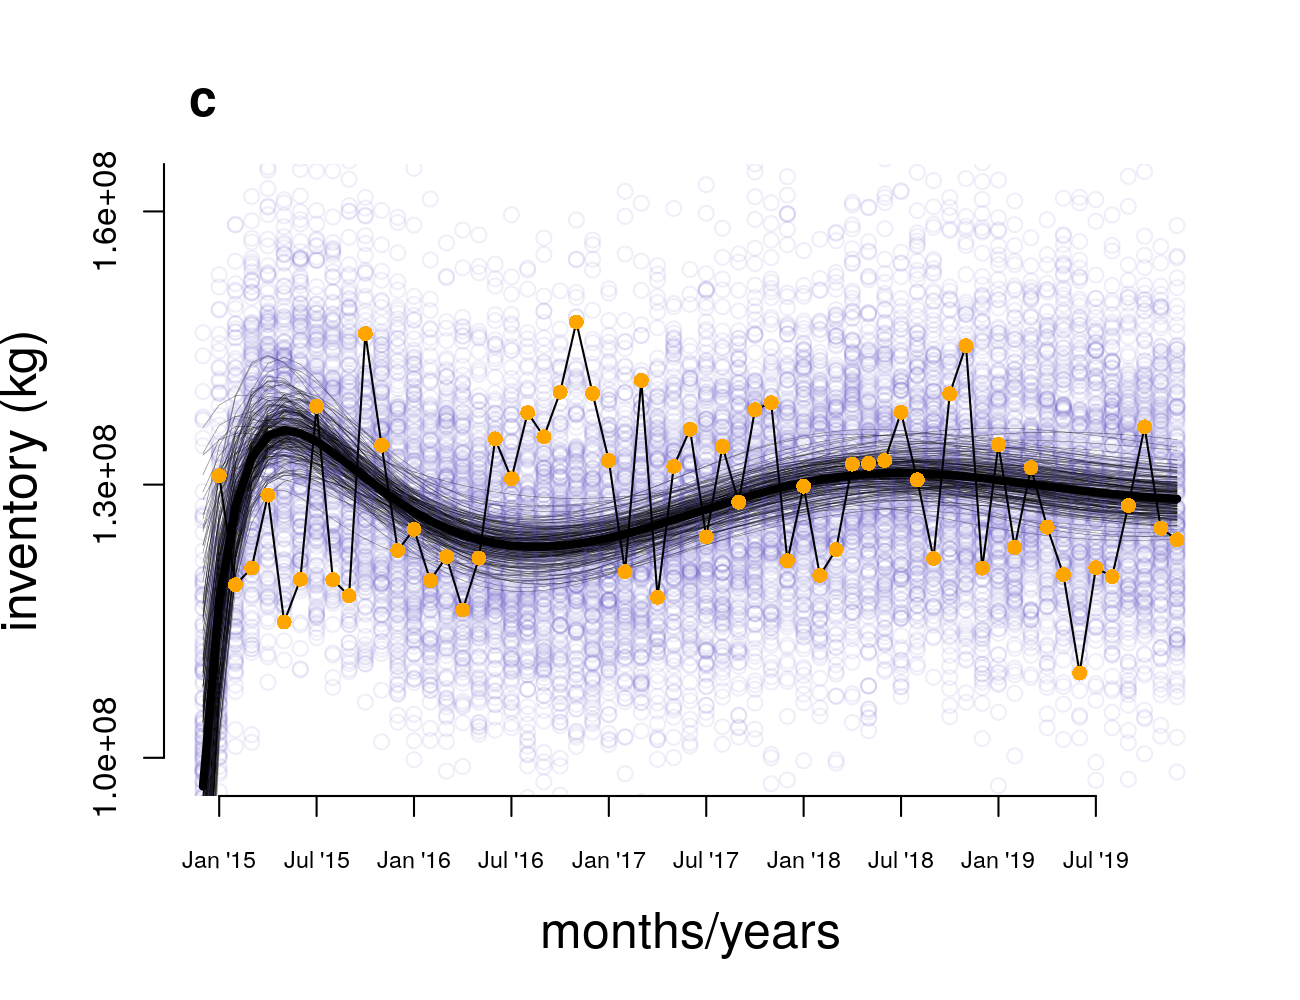
\includegraphics[scale=0.5]{figure_3c.png}
  \end{subfigure}%
  %~
  \begin{subfigure}{0.5\textwidth}
    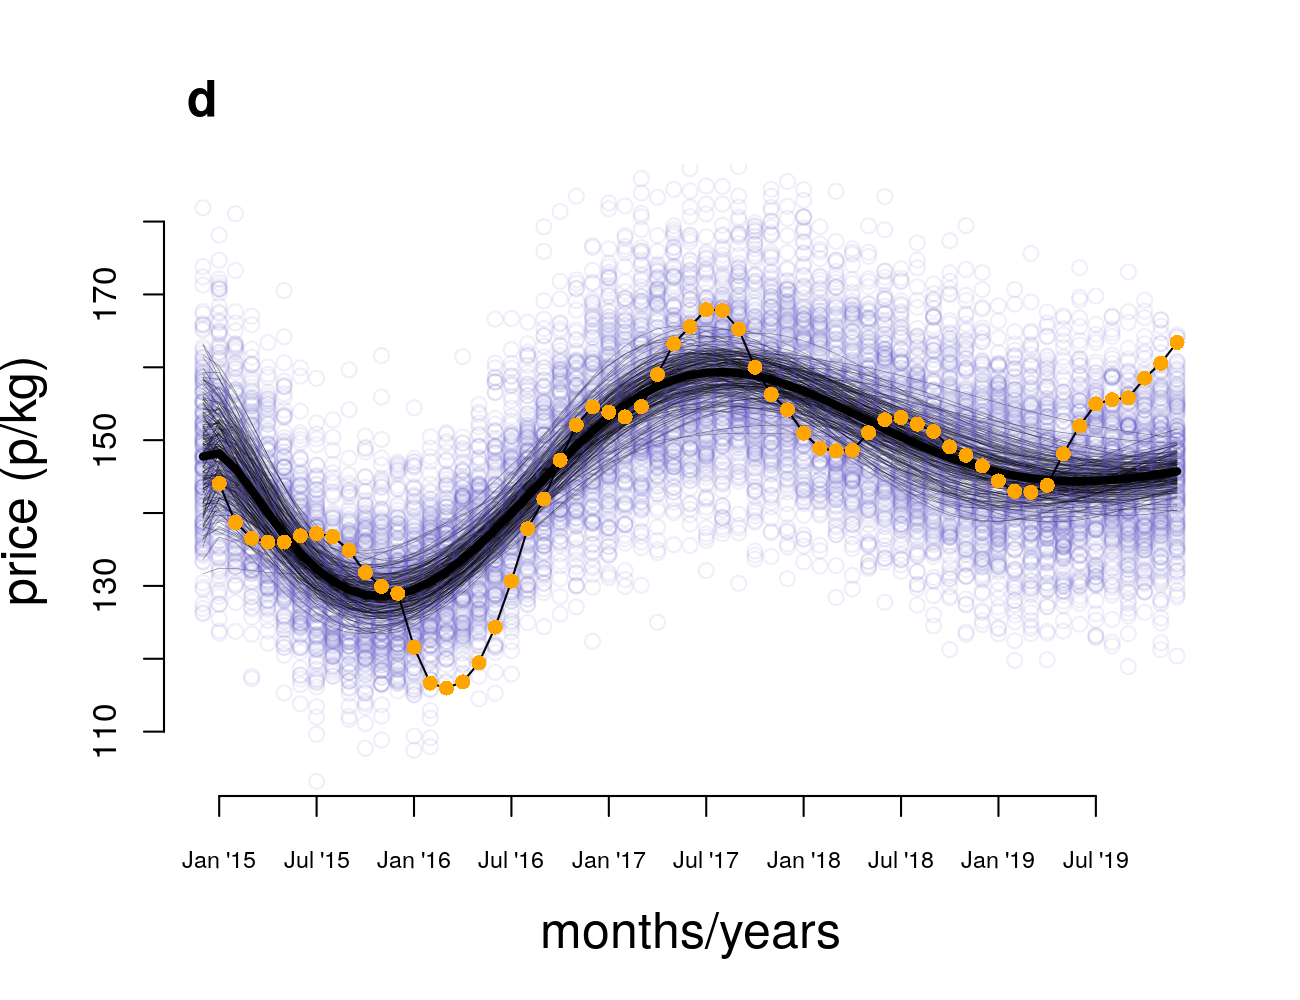
\includegraphics[scale=0.5]{figure_3d.png}
  \end{subfigure}

  \begin{subfigure}{0.5\textwidth}
    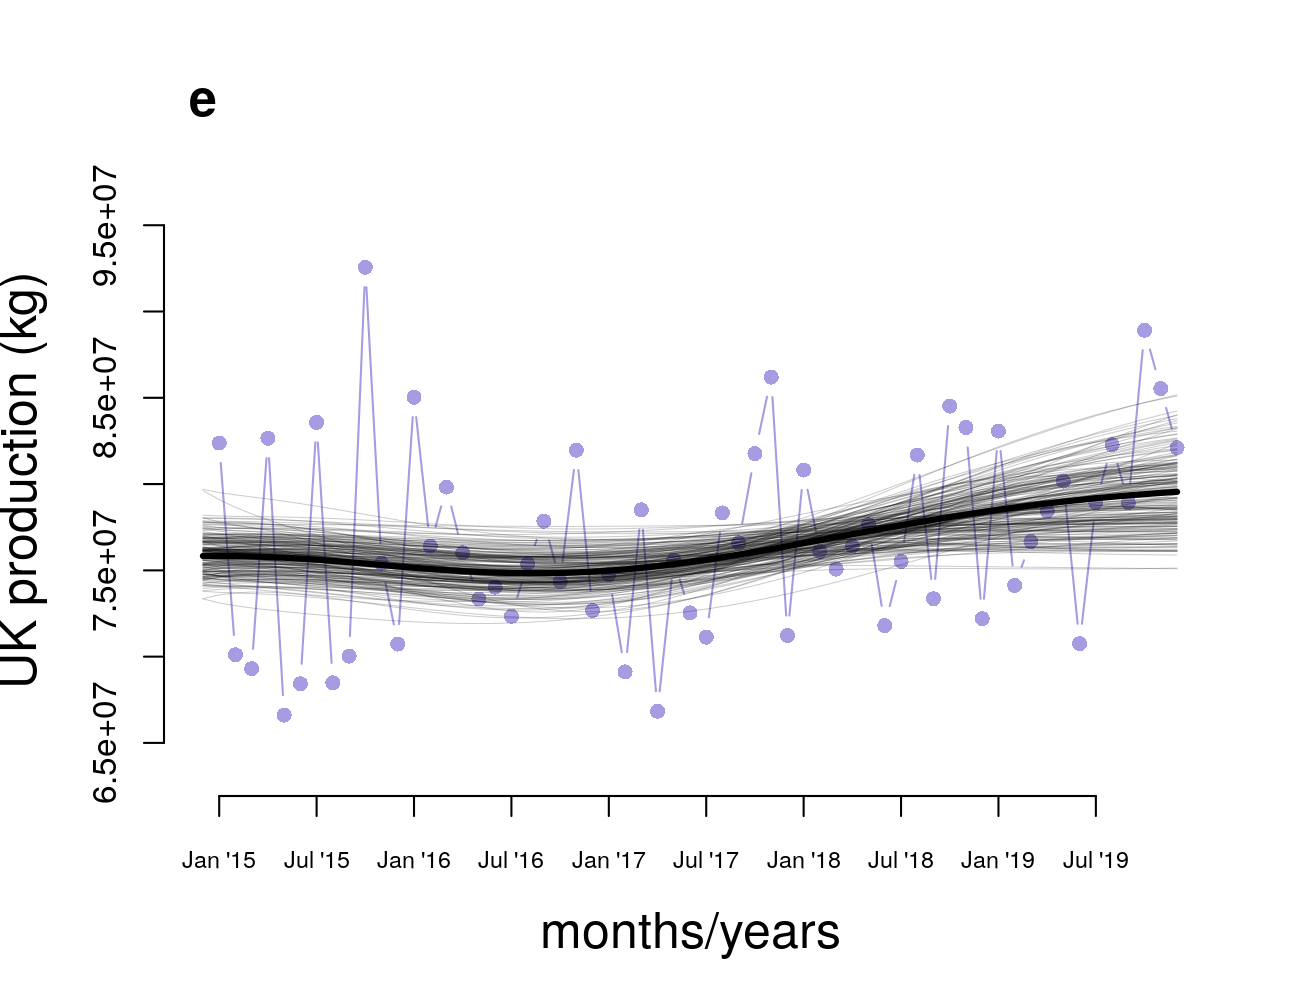
\includegraphics[scale=0.5]{figure_3e.png}
  \end{subfigure}%
  %~
  \begin{subfigure}{0.5\textwidth}
    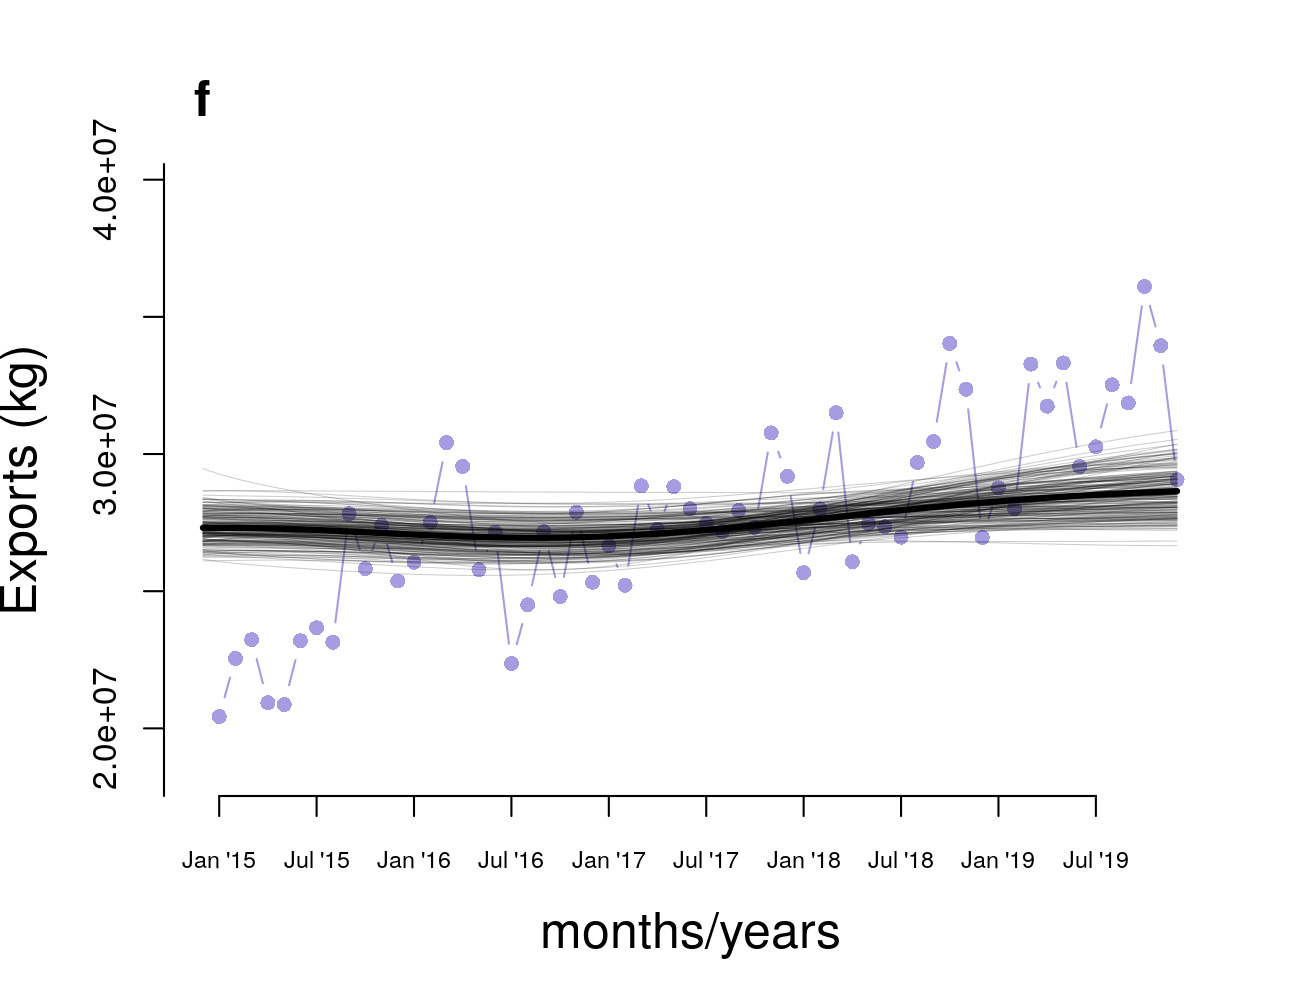
\includegraphics[scale=0.5]{figure_3f.png}
  \end{subfigure}
  \caption{Fitting the food systems model to the UK pig industry data. Blue dots show the raw monthly data (some data is missing), thin black lines display 200 random samples from the posterior distribution, and thick black lines indicate the mean posterior trajectory.}
\end{figure}

\section{Discussion}

\subsection{Limitations}


\newpage
\printbibliography
\end{document}
